\documentclass{article}
\usepackage{amssymb}
\usepackage{amsmath}
\usepackage{fancyhdr}
\usepackage{booktabs}
\usepackage{harvard}
\usepackage[hidelinks]{hyperref}
\citationmode{abbr}
\citationstyle{dcu}
\pagestyle{fancy}
\usepackage{graphicx}
\graphicspath{ {images/} }
\lhead{Justin Coker | Problem Set 8}
\rhead{}
\begin{document}
The equilibrium wage found by running the enclosed ps8.py is: 0.914873718262

The stationary Distribution:
\begin{center}
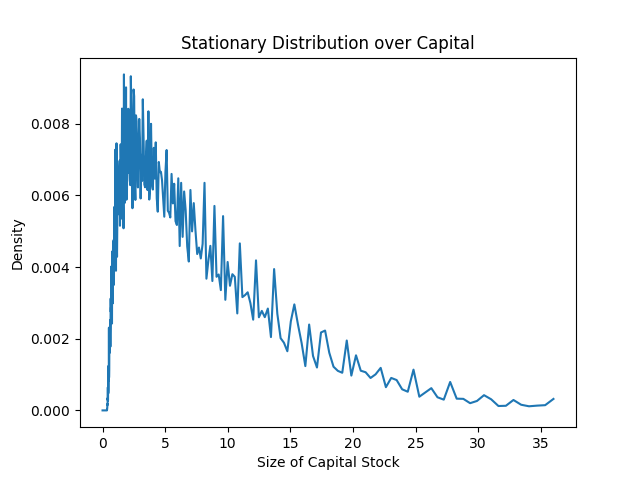
\includegraphics[scale = .65]{dist}
\end{center}

The policy functions:
\begin{center}
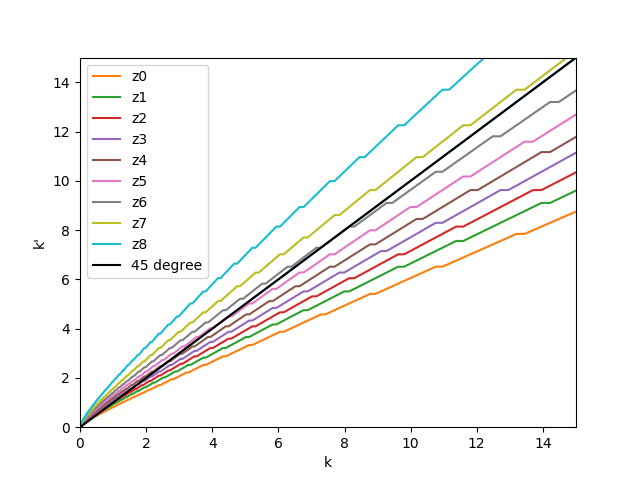
\includegraphics[scale = .65]{policy}
\end{center}
\newpage

When productivity is high (z8), the policy function is above the 45-degree line indicating that we should increase capital if productivity is high.
As productivity falls, the policy function also falls. This indicates that the optimal choice  of next period capital rises(falls) as productivity rises(falls) for any given current period capital stock.\\

Note that the graph's axes do not span the full range of capital. This is done so that the various productivity levels are distinguishable in the figure. 
\end{document}